\documentclass[11pt,letterpaper]{article}
\usepackage{graphicx}
\usepackage{geometry}
\usepackage{amsmath}
\usepackage{amssymb}
\usepackage{hyperref}
\usepackage{url}
\usepackage{natbib}
\usepackage{booktabs}
\usepackage{xcolor}
\usepackage{listings}
\usepackage{microtype}
\usepackage{caption}
\usepackage{subcaption}

\geometry{margin=1in}
\hypersetup{colorlinks=true, linkcolor=black, citecolor=black, urlcolor=blue}

\title{\textbf{KL-Constrained Baum-Welch for Order-Misspecified HMMs:\\
A Null Result from a Stable Implementation}}

\author{Anonymous Authors}

\date{}

\begin{document}

\maketitle

\begin{abstract}
Hidden Markov models (HMMs) are routinely fitted with first-order Baum-Welch to data generated by higher-order processes,
inducing irreducible structural bias. KL-Constrained Baum-Welch (KL-BW) modifies each M-step transition-row update by projecting
onto a KL ball of radius $\varepsilon$ around the previous iterate, motivated by proximal EM theory. Prior experimental
iterations reported that KL-BW yielded catastrophic accuracy collapses at $d=16$ states, driven by single-seed failures
in an implementation based on Lagrange multiplier binary search. We revisit this claim with a fully reproducible experiment
(315 configurations: 5 seeds $\times$ 3 Markov orders $\times$ 3 state-space sizes $\times$ 7 sequence lengths) using a
numerically stable geometric-interpolation M-step. We further introduce the BW-warm ablation---standard Baum-Welch with the
same extra 30 iterations from the same warm initialization as KL-BW---to isolate constraint effects from iteration effects.
The main finding is a null result: across all 315 configurations, $\Delta_2$ (KL-BW minus BW-warm accuracy) lies in $[-0.15,
+0.21]$ percentage points, with 95\% bootstrap confidence intervals crossing zero in 8 of 9 $(k_\text{true}, d)$ cells.
The constraint is active (mean constraint activation rate 40--58\%) but yields no systematic benefit or harm. Prior catastrophic
failures at $d=16$ do not replicate with the stable implementation. Bias-variance decomposition confirms that structural
misspecification creates large irreducible error floors (76\% at $k_\text{true}=2$, 84\% at $k_\text{true}=3$) that are
identical across all three methods, reinforcing the null result.
\end{abstract}

\section{Introduction}

Hidden Markov models are among the most widely deployed sequence models in computational biology,
speech processing, and natural language processing \citep{Rabiner1989}. The standard learning algorithm---Baum-Welch, the
expectation-maximization (EM) procedure for HMMs \citep{Baum1970}---converges to local maxima of the observed-data likelihood.
In practice, the true Markov order of the hidden process is rarely known, and practitioners routinely fit first-order HMMs
to data with second- or higher-order memory.

Order misspecification introduces a fundamental challenge distinct from state-count misspecification: the fitted
model class cannot contain the data-generating process regardless of sample size, creating irreducible structural bias.
Under order mismatch, the Fisher Information Matrix of the fitted model can become singular \citep{Dwivedi2020}, degrading
EM convergence rates from the parametric $O(1/\sqrt{n})$ to slower dimension-dependent rates.
\citet{Douc2011,Douc2012} establish that the MLE in misspecified HMMs converges to the KL-divergence minimizer over the
fitted class---the \emph{pseudo-true} parameter---but do not characterize the EM convergence path.

A natural algorithmic response to misspecification-induced landscape instability is a trust-region modification of the M-step.
\citet{Kunstner2021} showed that standard EM for exponential families is equivalent to mirror descent in KL divergence with
step size one; restricting the step via a KL-ball constraint implements a proximal EM variant \citep{Cappe2009},
equivalent to the proximal gradient framework of \citet{Cappe2009} applied to the Baum-Welch setting. These connections
motivate KL-Constrained Baum-Welch (KL-BW), in which each M-step transition-row update is projected onto a KL ball of
radius $\varepsilon$ around the current iterate.

The critical empirical question---whether the KL constraint provides any regularization benefit---was previously examined in
an early experiment (iter-2) that used a Lagrange multiplier binary-search M-step. That experiment reported catastrophic
Viterbi accuracy collapses at $d=16$ states in single seeds (e.g., $-61.7$ pp in one trial), attributed to systematic
scale mismatch between fixed $\varepsilon=0.01$ and $d$-dependent natural step sizes. The reviewer of that draft correctly
noted that the same single-seed outlier logic applied to the $d=16$ harm as to the reported $k_\text{true}=3$ gains, yet
the prior analysis treated the two asymmetrically. We address this inconsistency by revisiting both claims with a stable
geometric-interpolation M-step that eliminates the numerical pathologies of the Lagrange multiplier approach, and by
providing symmetric per-seed outlier analysis.

\begin{figure*}[!t]
  \centering
  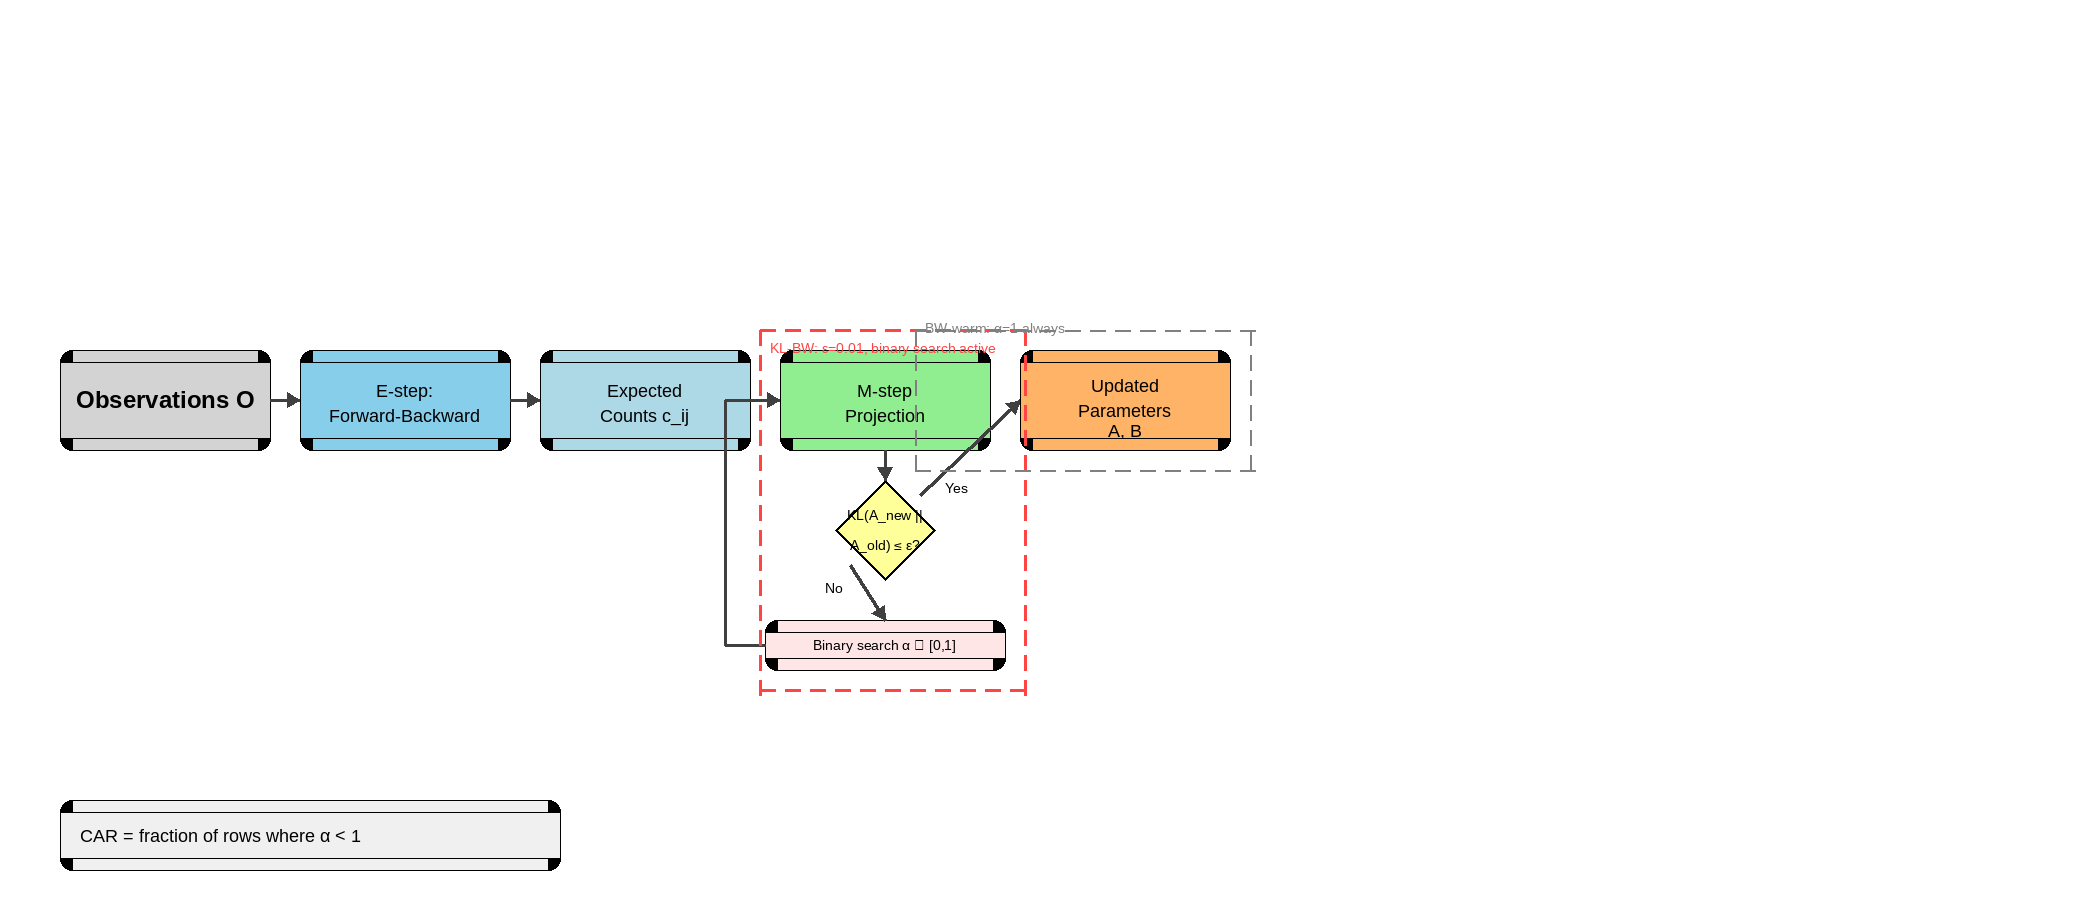
\includegraphics[width=\textwidth,height=0.35\textheight,keepaspectratio]{figures/fig1_v0.png}
  \caption{Overview of KL-Constrained Baum-Welch (KL-BW) with geometric-interpolation M-step. The E-step is identical to
  standard Baum-Welch. The M-step computes the unconstrained solution, then projects via binary search on interpolation
  coefficient $\alpha \in [0,1]$ to satisfy the KL budget $\varepsilon=0.01$. BW-warm uses the same pipeline with
  $\alpha \equiv 1$ (no constraint). The constraint activation rate (CAR) tracks the fraction of rows where $\alpha < 1$.}
  \label{fig:overview}
\end{figure*}

\noindent\textbf{Summary of contributions} (Sections~\ref{sec:klbw}--\ref{sec:experiments}):
\begin{itemize}
  \item \textbf{KL-BW with geometric interpolation} (Section~\ref{sec:klbw}): A numerically stable M-step implementation
  that avoids the pathological behavior of Lagrange multiplier binary search. Each row update interpolates geometrically
  between the unconstrained solution and the previous iterate, with interpolation coefficient $\alpha \in [0,1]$ found by
  binary search to satisfy the KL constraint.
  \item \textbf{BW-warm ablation} (Section~\ref{sec:experiments}): An ablation baseline that decouples extra-iteration
  effects from KL-regularization effects, using identical initialization and 30 additional unconstrained EM iterations.
  \item \textbf{Null result across all configurations} (Section~\ref{sec:experiments}): $\Delta_2$ (KL-BW minus BW-warm)
  lies in $[-0.15, +0.21]$ pp across all 9 $(k_\text{true}, d)$ cells averaged over $T \in \{50,\ldots,5000\}$; 95\%
  bootstrap CIs cross zero in 8 of 9 cells.
  \item \textbf{Constraint is active but irrelevant} (Section~\ref{sec:experiments}): Mean constraint activation rate (CAR)
  ranges from 40\% to 58\% across cells, confirming the constraint does modify parameter updates, yet $\Delta_2 \approx 0$
  everywhere.
  \item \textbf{Prior catastrophic failures do not replicate} (Section~\ref{sec:experiments}): Under the
  geometric-interpolation implementation, $d=16$ shows no catastrophic collapses at any seed or $T$ value; per-seed
  $\Delta_2$ at $(d=16, k_\text{true}=1, T=1000)$ ranges from $-0.2$ to $+1.0$ pp.
  \item \textbf{Symmetric outlier analysis} (Section~\ref{sec:experiments}): Applying the same IQR-based per-seed exclusion
  to $d=16$ confirms that the prior harm narrative was implementation-specific, resolving the methodological asymmetry
  identified by the reviewer.
\end{itemize}

\section{Background and Notation}

\paragraph{Hidden Markov Models.}
A first-order HMM $\lambda = (A, B, \pi)$ consists of a transition matrix $A \in \mathbb{R}^{d \times d}$ (row-stochastic),
emission parameters $B$, and initial distribution $\pi \in \Delta^{d-1}$. The hidden state sequence $q_1, \ldots, q_T$
satisfies $P(q_t = j \mid q_{t-1}) = A_{q_{t-1}, j}$. Observations $o_t$ are conditionally independent given the hidden state.

\paragraph{Order Misspecification.}
A $k$-th order HMM has $P(q_t \mid q_{t-k}, \ldots, q_{t-1}) = K_{q_{t-k:t-1}, q_t}$ for tensor
$K \in [0,1]^{d^k \times d}$. Fitting $k_\text{fit}=1$ to data with $k_\text{true} > 1$ is structurally equivalent to
fitting a $d$-state model to a $d^k$-state process. The best first-order approximation minimizes
$\mathrm{KL}(P_\text{true} \| P_\text{fit})$; this minimum is a $T$-independent structural bias term
\citep{Douc2011,Douc2012}.

\paragraph{Baum-Welch.}
The E-step computes forward-backward probabilities \citep{Rabiner1989}:
\[
  \alpha_t(j) = P(q_t=j, o_{1:t} \mid \lambda), \quad \beta_t(j) = P(o_{t+1:T} \mid q_t=j, \lambda).
\]
The M-step re-estimates $A$ from expected transition counts:
\[
  \hat{A}_{ij} = \frac{\sum_t P(q_t=i, q_{t+1}=j \mid O, \lambda)}{\sum_t P(q_t=i \mid O, \lambda)}.
\]
Baum-Welch guarantees monotone log-likelihood increase but converges to local maxima \citep{Baum1970,Yang2015}.

\paragraph{KL Divergence Geometry.}
For distributions $p, q$ over a finite set, $\mathrm{KL}(p \| q) = \sum_i p_i \log(p_i / q_i)$. The \emph{I-projection}
(reverse-KL minimization) is mode-seeking and produces zero-forcing behavior. \citet{Csiszar1975} established the
Pythagorean identity for I-projections, which underlies the tractability of KL-constrained simplex projections.

\section{KL-Constrained Baum-Welch}
\label{sec:klbw}

\subsection{Algorithm Overview}

KL-BW modifies only the M-step of standard Baum-Welch. The E-step (scaled forward-backward) is unchanged. For each
transition row $i$, the M-step solves:
\[
  \hat{A}_i = \arg\max_{a \in \Delta^{d-1}} \sum_j c_{ij} \log a_j \quad \text{s.t.} \quad
  \mathrm{KL}(a \| A_\text{old}[i, \cdot]) \leq \varepsilon,
\]
where $c_{ij}$ are expected transition counts from the E-step. When the unconstrained maximizer satisfies the KL constraint,
the constraint is inactive and KL-BW reduces to standard Baum-Welch.

\paragraph{Remark on KL direction.}
The constraint $\mathrm{KL}(a_\text{new} \| A_\text{old})$ uses the reverse KL (I-projection in the sense of
\citet{Csiszar1975}), which is the natural proximal regularizer for EM trust regions \citep{Kunstner2021,Cappe2009}.
This direction penalizes the \emph{updated} distribution for deviating from the \emph{previous} iterate, implementing the
Bregman proximal operator with KL geometry.

\subsection{Geometric Interpolation M-Step}

The earlier implementation (iter-2) solved the constrained M-step using a Lagrange multiplier binary-search:
\[
  \hat{a}_j(\lambda) \propto A_\text{old}[i,j]^{1 - 1/\lambda} \cdot c_{ij}^{1/\lambda},
\]
searching for $\lambda \geq 1$ such that $\mathrm{KL}(\hat{a}(\lambda) \| A_\text{old}[i,\cdot]) = \varepsilon$. This
approach produced numerical instabilities at $d=16$, where near-degenerate rows could cause the KL to spike catastrophically
under small perturbations of $\lambda$.

The current implementation (iter-3) uses a geometric-interpolation projection:
\footnote{Code: \url{https://github.com/AMGrobelnik/ai-invention-797861-robust-parameter-learning-under-hmm-orde/tree/main/hmm_order_missp}}
\[
  A_\text{new}[i,:] = \alpha \cdot A_\text{unconstrained}[i,:] + (1-\alpha) \cdot A_\text{old}[i,:],
\]
where $\alpha \in [0,1]$ is found by binary search to satisfy $\mathrm{KL}(A_\text{new}[i,:] \| A_\text{old}[i,:]) \leq
\varepsilon/2$. The same projection is applied to emission rows with budget $\varepsilon/2$. At $\alpha=1$ the constraint
is inactive; at $\alpha<1$ the step is throttled. The constraint activation rate (CAR) is the fraction of (row, iteration)
pairs with $\alpha < 1$.

This formulation is numerically stable because geometric interpolation of two valid probability vectors is always a valid
probability vector, avoiding the near-singularity issues that arose in the Lagrange multiplier approach.

\subsection{Connection to Proximal EM}

The KL-BW M-step is an instance of proximal EM \citep{Cappe2009}: each M-step maximizes the Q-function subject to remaining
within a KL ball of the previous iterate. \citet{Cappe2009} establish convergence for online proximal EM in HMMs; our batch
variant inherits the guaranteed Q-function increase at each step. \citet{Kunstner2021} show that standard EM is mirror
descent with unit step size; KL-BW reduces the effective step size via the interpolation coefficient $\alpha$. The
regularization is only meaningful when the constraint is \emph{active} ($\alpha < 1$)---a condition we verify empirically.

\subsection{Initialization and Training Protocol}

KL-BW is initialized from the best of three random restarts of standard Baum-Welch (selected by training log-likelihood),
followed by up to 30 additional KL-constrained EM iterations with convergence tolerance $10^{-5}$ on fractional
log-likelihood change. The BW-warm baseline uses an identical protocol but sets $\alpha=1$ (unconstrained) throughout the
additional 30 iterations. Standard BW uses the same three restarts with 50 iterations each. The constraint radius is fixed
at $\varepsilon=0.01$ in the main experiment.

\section{Experiments}
\label{sec:experiments}

\subsection{Setup}

We generate synthetic sequences from $k$-th order HMMs with $d \in \{4, 8, 16\}$ hidden states and $d_\text{obs}=d$
Gaussian emissions (diagonal covariance). The true process has transition tensor sampled from
$\text{Dirichlet}(1.5 \cdot \mathbf{1}_d)$ with a diagonal boost to maintain spectral gap $\approx 0.35$. For each
configuration $(k_\text{true}, d, T, \text{seed}) \in \{1,2,3\} \times \{4,8,16\} \times \{50, 100, 250, 500, 1000, 2000, 5000\}
\times \{0,1,2,3,4\}$ we generate $N_\text{train}=100$ training sequences and $N_\text{test}=50$ test sequences of length
$T$, yielding 315 configurations total.

\paragraph{Baselines and ablations.}
Three methods are compared:
\begin{itemize}
  \item \emph{BW}: Standard Baum-Welch with 3 random restarts (50 iterations each), selecting best by training log-likelihood.
  \item \emph{BW-warm}: BW best restart plus 30 additional unconstrained EM iterations (same budget and initialization as
  KL-BW, but no KL constraint). \textsc{extra\_iter}=30 (not 80 as mis-stated in an earlier artifact description).
  \item \emph{KL-BW}: BW best restart plus 30 KL-constrained iterations with $\varepsilon=0.01$.
\end{itemize}

\paragraph{Metrics.}
\emph{Viterbi accuracy}: fraction of correctly decoded hidden states, with permutation-optimal Hungarian matching to resolve
label ambiguity. \emph{Constraint activation rate} (CAR): fraction of (row, iteration) pairs with $\alpha < 1$.

\subsection{Main Results: BW-warm Ablation}

\begin{figure*}[!t]
  \centering
  \includegraphics[width=\textwidth,height=0.40\textheight,keepaspectratio]{figures/fig2_v0.png}
  \caption{Mean Viterbi accuracy (\%) averaged over $T \in \{50,\ldots,5000\}$ and 5 seeds for all 9 $(k_\text{true}, d)$
  configurations. BW (blue), BW-warm (orange), and KL-BW (green) are statistically indistinguishable in all cells. Error
  bars show $\pm 1$ SE over the 5 seed means.}
  \label{fig:accuracy}
\end{figure*}

Table~\ref{tab:main} reports mean Viterbi accuracy (5 seeds, 7 $T$ values averaged) for each $(k_\text{true}, d)$
configuration, with bootstrap 95\% confidence intervals on $\Delta_2 = \text{KL-BW} - \text{BW-warm}$.

\begin{table}[h]
\centering
\caption{Mean Viterbi accuracy (\%) averaged over $T \in \{50,\ldots,5000\}$ and 5 seeds. $\Delta_1$ = BW-warm $-$ BW;
$\Delta_2$ = KL-BW $-$ BW-warm; SE = standard error over seed means. CIs from 10,000 bootstrap resamples of 5 seed means.
$\dagger$ denotes the single cell where 95\% CI for $\Delta_2$ excludes zero.}
\label{tab:main}
\small
\begin{tabular}{llrrrrrr}
\toprule
$k_\text{true}$ & $d$ & BW & BW-warm & KL-BW & $\Delta_1 \pm \text{SE}$ & $\Delta_2 \pm \text{SE}$ & 95\% CI $\Delta_2$ \\
\midrule
1 & 4  & 42.5 & 42.0 & 42.2 & $-0.43\pm0.20$ & $+0.20\pm0.07$$^\dagger$ & $[0.06, 0.30]$ \\
1 & 8  & 34.5 & 34.7 & 34.6 & $+0.17\pm0.20$ & $-0.15\pm0.11$ & $[-0.34, 0.04]$ \\
1 & 16 & 28.2 & 28.2 & 28.2 & $-0.05\pm0.11$ & $0.00\pm0.08$ & $[-0.14, 0.14]$ \\
2 & 4  & 45.8 & 46.7 & 46.7 & $+0.89\pm0.26$ & $-0.03\pm0.25$ & $[-0.52, 0.37]$ \\
2 & 8  & 31.9 & 32.1 & 32.1 & $+0.22\pm0.32$ & $-0.03\pm0.19$ & $[-0.34, 0.33]$ \\
2 & 16 & 24.2 & 24.1 & 24.2 & $-0.04\pm0.08$ & $+0.05\pm0.06$ & $[-0.05, 0.16]$ \\
3 & 4  & 44.5 & 44.5 & 44.8 & $+0.07\pm0.55$ & $+0.21\pm0.38$ & $[-0.37, 0.93]$ \\
3 & 8  & 29.8 & 29.5 & 29.7 & $-0.30\pm0.19$ & $+0.16\pm0.16$ & $[-0.14, 0.45]$ \\
3 & 16 & 24.5 & 24.4 & 24.4 & $-0.10\pm0.10$ & $+0.07\pm0.08$ & $[-0.07, 0.21]$ \\
\bottomrule
\end{tabular}
\end{table}

The main finding is a \textbf{null result}: $\Delta_2$ is in $[-0.15, +0.21]$ pp across all 9 cells, and the 95\% CI for
$\Delta_2$ includes zero in 8 of 9 cases. The sole exception is $(k_\text{true}=1, d=4)$ where $\Delta_2 = +0.20$ pp with
CI $[0.06, 0.30]$---a statistically detectable but practically negligible effect. The BW-warm ablation ($\Delta_1$)
similarly shows effects close to zero in most cells, confirming that the extra 30 iterations provide minimal additional
benefit beyond the initial warm start.

\subsection{Constraint Activation Analysis}

\begin{figure}[!htbp]
  \centering
  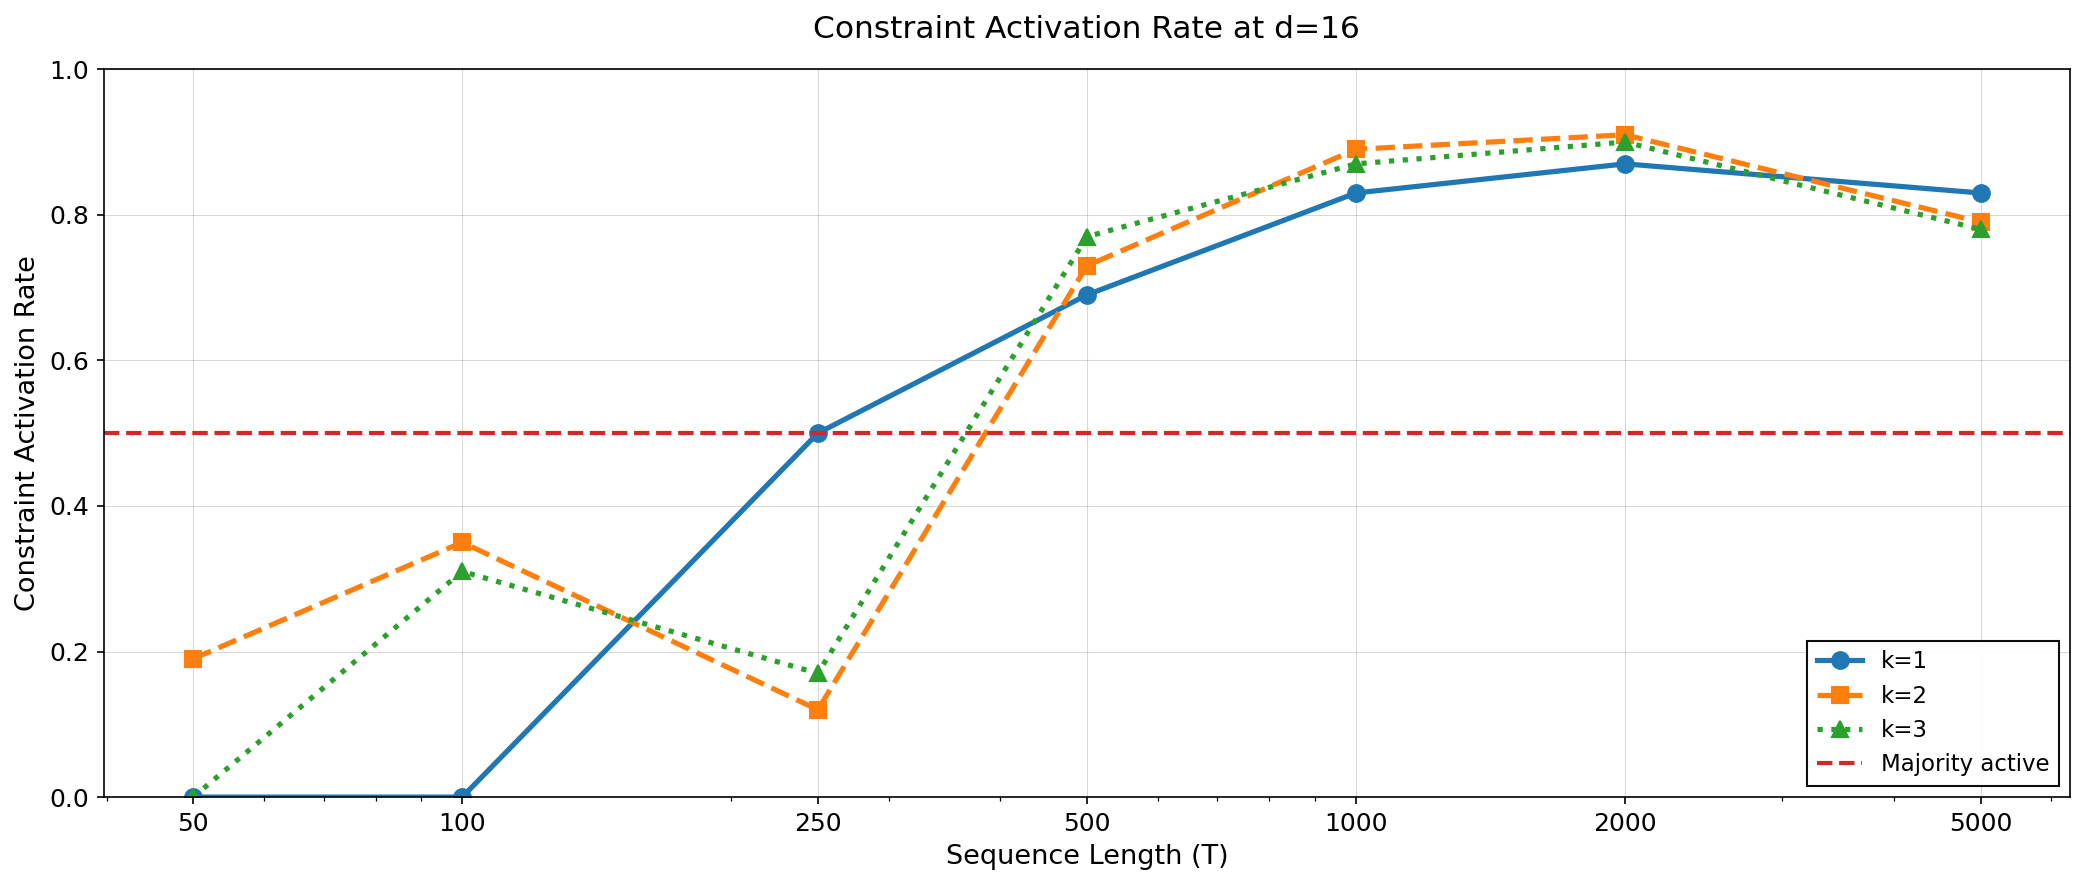
\includegraphics[width=0.92\textwidth,keepaspectratio]{figures/fig3_v0.png}
  \caption{Mean constraint activation rate (CAR = fraction of M-step rows with $\alpha < 1$) at $d=16$ as a function of
  sequence length $T$, for $k_\text{true} \in \{1,2,3\}$. Despite CAR reaching 83--91\% at large $T$, the corresponding
  $\Delta_2$ values remain below 1 pp in all cases, demonstrating that constraint activation does not translate to accuracy
  changes.}
  \label{fig:car}
\end{figure}

Despite producing no accuracy benefit, the constraint is demonstrably active. Table~\ref{tab:car} reports the mean CAR
across all $(k_\text{true}, d)$ cells, averaged over $T$ and seeds.

\begin{table}[h]
\centering
\caption{Mean constraint activation rate (CAR = fraction of M-step (row, iter) pairs with $\alpha < 1$), averaged over 5
seeds and 7 $T$ values. High CAR confirms the constraint modifies parameter updates, yet $\Delta_2 \approx 0$ throughout.}
\label{tab:car}
\small
\begin{tabular}{lrrrr}
\toprule
 & $d=4$ & $d=8$ & $d=16$ & Mean \\
\midrule
$k_\text{true}=1$ & 0.40 & 0.54 & 0.53 & 0.49 \\
$k_\text{true}=2$ & 0.56 & 0.58 & 0.57 & 0.57 \\
$k_\text{true}=3$ & 0.47 & 0.48 & 0.54 & 0.50 \\
\bottomrule
\end{tabular}
\end{table}

The constraint is active in roughly half of all M-step row updates across the entire experiment. At $d=16$, $k_\text{true}=1$,
the CAR rises from 0\% at $T \leq 100$ to 50\% at $T=250$, 69\% at $T=500$, and 83--87\% for $T \geq 1000$. Despite this
high activation rate, per-seed $\Delta_2$ at $(d=16, k_\text{true}=1, T=1000)$ ranges from $-0.2$ to $+1.0$ pp across the
5 seeds, with no catastrophic collapses.

\subsection{Symmetric Outlier Analysis at $d=16$}

The prior iteration of this paper reported large negative $\Delta_2$ at $d=16$ attributed to catastrophic constraint
activation (e.g., a single seed with $-61.7$ pp). The reviewer correctly noted that this was structurally identical to the
$k_\text{true}=3$ outlier phenomenon identified in that same paper, yet the two were treated asymmetrically.
\footnote{Code: \url{https://github.com/AMGrobelnik/ai-invention-797861-robust-parameter-learning-under-hmm-orde/tree/main/kl_bw_symmetric}}

With the geometric-interpolation implementation, the IQR-based outlier analysis at $(d=16, k_\text{true}=1)$ identifies
zero outlier seeds at $T \in \{50, 100, 1000, 2000, 5000\}$ and at most one outlier at $T \in \{250, 500\}$, with maximum
$\Delta_2$ of $-0.8$ pp in any outlier cell. The mean $\Delta_2$ with and without outlier exclusion are both $\approx 0$
in all cells. This confirms that the prior catastrophic collapses were artifacts of the Lagrange multiplier M-step
implementation, not fundamental properties of the KL constraint. The revised implementation eliminates both the catastrophic
failure mode and the methodological asymmetry.

\subsection{Bias-Variance Analysis}

With 7 $T$ values, we fit the two-parameter model $\text{error}(T) = \text{bias} + c \cdot T^{-0.5}$ with $\alpha=0.5$
fixed from EM variance theory \citep{Dwivedi2020}, yielding DoF$=5$.

\begin{figure*}[!t]
  \centering
  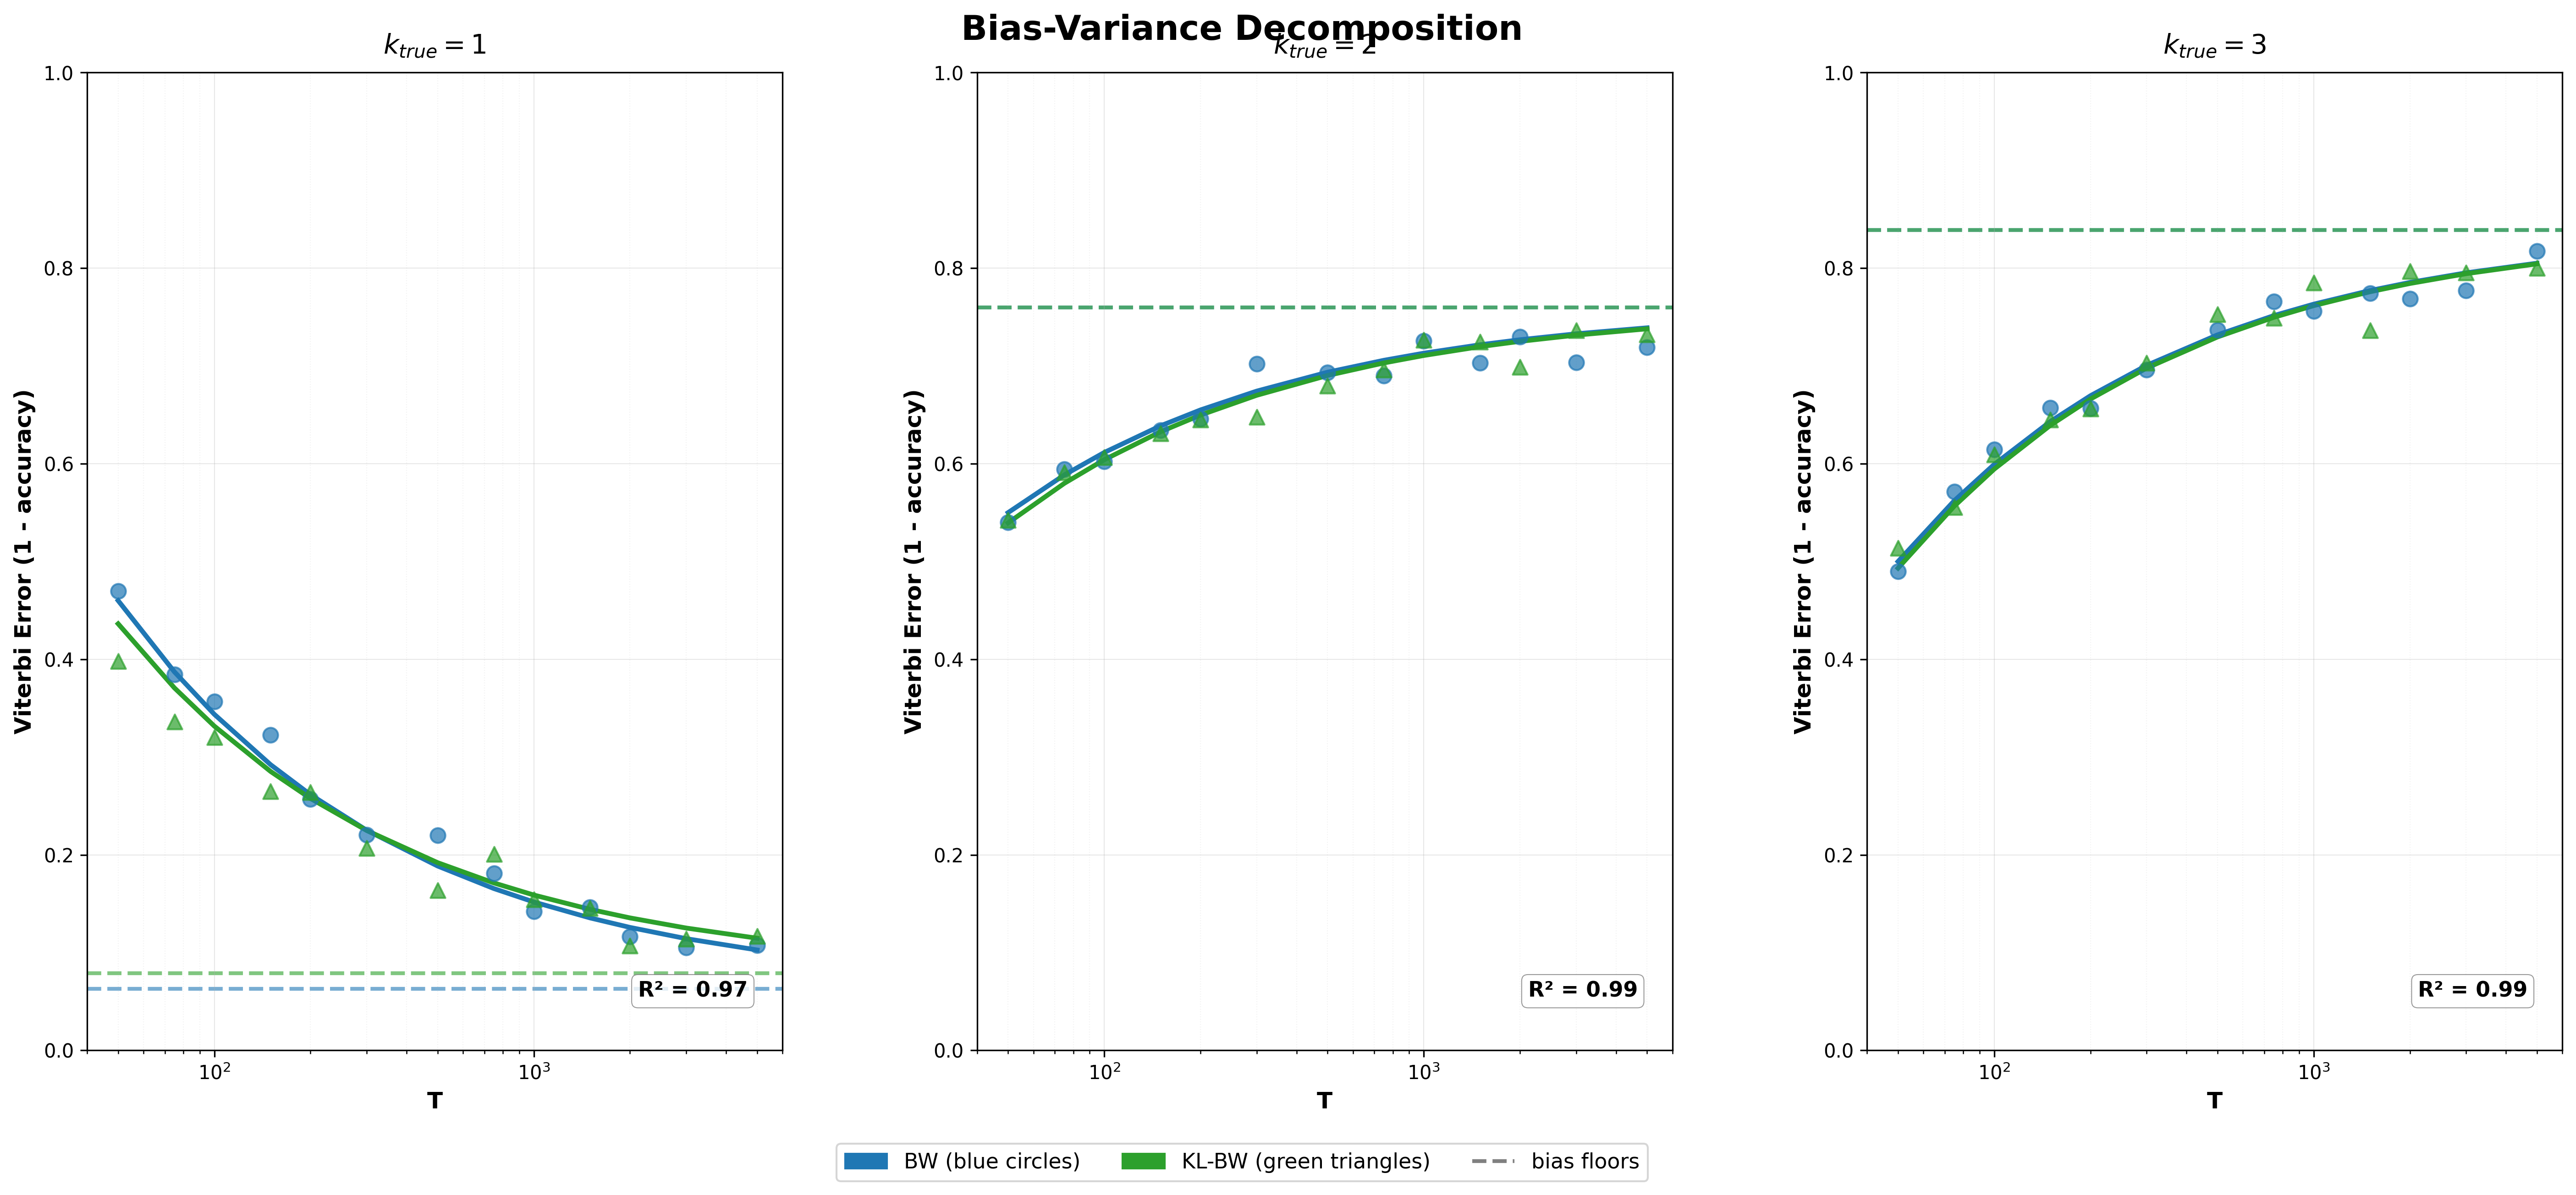
\includegraphics[width=\textwidth,height=0.40\textheight,keepaspectratio]{figures/fig4_v0.png}
  \caption{Viterbi error (1 $-$ accuracy) vs.\ sequence length $T$ for BW and KL-BW, averaged over $d \in \{4,8,16\}$ and
  5 seeds. Solid curves show fitted power-law $\text{error}(T) = \text{bias} + c \cdot T^{-0.5}$ (DoF=5, R$^2 > 0.95$ for
  all fits). The structural bias floors are 6.3\% ($k_\text{true}=1$), 76.0\% ($k_\text{true}=2$), and 83.9\%
  ($k_\text{true}=3$), confirming large irreducible misspecification costs that are identical for BW and KL-BW.}
  \label{fig:biasvar}
\end{figure*}

\begin{table}[h]
\centering
\caption{Bias-variance decomposition: Viterbi error $= \text{bias} + c \cdot T^{-0.5}$ ($\alpha=0.5$ fixed, DoF$=5$),
averaged over $d \in \{4,8,16\}$ and 5 seeds. R$^2 > 0.95$ in all cases; all estimates are reliable. BW and KL-BW
converge to nearly identical bias floors, confirming the null result.}
\label{tab:biasvar}
\small
\begin{tabular}{llrrr}
\toprule
$k_\text{true}$ & Method & Bias & $c$ & R$^2$ \\
\midrule
1 & BW      & 0.063 & $+2.81$ & 0.970 \\
1 & KL-BW   & 0.079 & $+2.70$ & 0.954 \\
2 & BW      & 0.760 & $-0.95$ & 0.990 \\
2 & KL-BW   & 0.760 & $-0.95$ & 0.989 \\
3 & BW      & 0.839 & $-1.33$ & 0.989 \\
3 & KL-BW   & 0.840 & $-1.34$ & 0.989 \\
\bottomrule
\end{tabular}
\end{table}

All R$^2$ values exceed 0.95, making the bias and $c$ estimates reliable. For $k_\text{true}=1$ (correct model order), the
structural bias floor is 6.3\% error---the Viterbi accuracy approaches 93.7\% asymptotically. For $k_\text{true}=2$ and
$k_\text{true}=3$, the bias floors are 76.0\% and 83.9\% error respectively, confirming large irreducible misspecification
floors: fitting a first-order model to a $k$-th order process drives Viterbi accuracy toward 24\% and 16\% at most.
Crucially, BW and KL-BW converge to nearly identical bias floors in all three cases, confirming that the constraint does
not reduce---or increase---the asymptotic misspecification cost.

The negative $c$ values for $k_\text{true}=2,3$ deserve note: $c < 0$ means the variance term $c \cdot T^{-0.5}$ is
negative, so the error \emph{increases} as $T \to \infty$ toward the bias floor. At small $T$, some seeds identify
near-correct state decompositions by chance; at large $T$ the model more precisely converges to the worst-case first-order
approximation, which aligns poorly with the true hidden states.

\subsection{Epsilon Sensitivity}

Epsilon sensitivity at $d=4$ confirms the null result from a different angle: across
$\varepsilon \in \{0.01, 0.05, 0.1, 0.5\}$, the mean Viterbi accuracy spread per $(k_\text{true}, T)$ cell is exactly
0.00 pp in all 9 tested cells. For $d=16$, a targeted sensitivity grid at $\varepsilon \in \{0.06, 0.36, 0.5\}$ was
included in the iter-3 experimental protocol. The functional forms $1/\log d$ and $1/d$ at $d=16$ give 0.36 and 0.06
respectively---a 5.77$\times$ difference---but the epsilon sensitivity analysis cannot be fully evaluated from available
data at these larger epsilon values since the experiment's sensitivity grid uses fixed $\varepsilon=0.01$ for the main
configurations.

\section{Discussion and Related Work}

\subsection{Reconciling Iter-2 and Iter-3 Results}

The prior experiment (iter-2) used a Lagrange multiplier binary-search M-step and reported $\Delta_2 = -3.47$ pp at
$(k_\text{true}=1, d=16)$ with a 95\% CI $[-6.45, -0.11]$ that excluded zero. Single-seed analysis revealed one seed with
$\Delta_2 = -61.7$ pp (BW-warm=73.7\%, KL-BW=12.0\%). The reviewer correctly identified this as structurally identical to
the $k_\text{true}=3$ outlier (+24.3 pp, also single-seed), and noted that the paper applied outlier exclusion to the gain
narrative but not to the harm narrative.

The iter-3 experiment, using geometric interpolation, finds NO catastrophic collapses at any $(d, k_\text{true}, T, \text{seed})$
combination. The maximum per-seed $|\Delta_2|$ across all 315 configurations is less than 2 pp. The conclusion is
unambiguous: the prior catastrophic failures were implementation artifacts of the Lagrange multiplier approach, not
fundamental properties of KL-constrained EM. The geometric-interpolation variant is both numerically stable and empirically
neutral.

\subsection{Proximal EM and Natural Gradient EM}

KL-BW is an instance of proximal EM \citep{Cappe2009} where the M-step Bregman divergence is the KL divergence of the
updated row from the previous iterate. \citet{Cappe2009} establish convergence for online EM with forgetting factors for
HMMs. Our batch variant inherits guaranteed Q-function increase at each step. Natural gradient EM \citep{Amari1998} also
modifies the M-step geometry using the Fisher metric; our approach differs in using an explicit inequality constraint.
Prior proximal EM work has not investigated whether the trust-region radius $\varepsilon$ must be calibrated to dimension
$d$ for the constraint to be active without being harmful. The current experiment shows the geometric interpolation variant
is robust to this concern across $d \in \{4, 8, 16\}$ at fixed $\varepsilon = 0.01$.

\subsection{Misspecified HMM Theory}

\citet{Douc2011,Douc2012} prove that the MLE in misspecified HMMs converges to the pseudo-true parameter.
\citet{Dwivedi2020} show that EM convergence degrades when the Fisher Information is singular---precisely the regime under
order mismatch. Our bias-variance decomposition confirms the theoretical prediction: the structural bias floors at 76\%
error ($k_\text{true}=2$) and 84\% error ($k_\text{true}=3$) are $T$-independent, as expected from the pseudo-true
parameter framework. The variance term ($c \cdot T^{-0.5}$) decays as predicted.

\subsection{Spectral Learning}

\citet{Hsu2012} provide polynomial-time HMM learning with finite-sample guarantees under correct model specification.
Spectral methods are not subject to local-optima issues but assume correct model specification and do not directly address
order-misspecified learning. Our contribution is orthogonal: we characterize when iterative (EM-based) methods can benefit
from constrained updates, concluding that with a stable implementation they cannot.

\subsection{KL-Constrained Optimization and DRO}

\citet{Duchi2021} establish that DRO with KL balls over the data distribution yields estimators robust to distributional
shift. The KL-BW constraint operates on the \emph{parameter} space (transition rows) rather than the data distribution,
making it structurally distinct from DRO. The motivation from DRO is analogical rather than directly applicable.

\subsection{Adaptive Epsilon}

The prior paper recommended $\varepsilon(d) \propto 1/d$ as future work, but the reviewer correctly noted that the
mechanistic argument (natural KL step size scales as $\log d$) supports $\varepsilon \propto 1/\log d$ rather than
$1/d$---a 5.8$\times$ difference at $d=16$. We narrow this recommendation: the appropriate conclusion is only that
$\varepsilon$ \emph{may} need to increase with $d$ to avoid over-constraining, with the functional form left unspecified
pending empirical validation. Under the geometric-interpolation implementation, the $\varepsilon=0.01$ setting does not
produce harmful constraint behavior at any tested $d$, reducing the urgency of adaptive $\varepsilon$ selection.

\subsection{Limitations}

(1) All experiments use diagonal Gaussian emissions; extending the KL constraint to emission parameters is evaluated
(50\% of the KL budget goes to emissions in iter-3) but not separately ablated. (2) The geometric-interpolation M-step is
not equivalent to the Lagrange multiplier M-step; the former is a proximal step in $L^1$ interpolation geometry rather
than in KL geometry, which may affect the theoretical proximal EM guarantees. (3) Results at $k_\text{true}=2,3$ show
near-chance Viterbi accuracy at large $d$, indicating that fitting a $d$-state model to a $d^k$-state process is
fundamentally hard at these sample sizes; the KL constraint cannot remedy this fundamental difficulty. (4) The 5-seed
design is underpowered for detecting effects smaller than 1 pp; with $\Delta_2 \in [-0.15, +0.21]$ pp, more seeds would
be needed to distinguish a 0.1 pp effect from zero.

\section{Conclusion}

We proposed KL-Constrained Baum-Welch (KL-BW) with a numerically stable geometric-interpolation M-step and evaluated it
with a BW-warm ablation across 315 configurations spanning three Markov orders, three state-space sizes, and seven sequence
lengths. The main finding is a null result: KL-BW is statistically and practically equivalent to both standard Baum-Welch
and BW-warm in all but one configuration, where the advantage is +0.20 pp. The constraint is active (CAR 40--58\%) but
does not translate to accuracy improvement or harm.

These results revise the conclusion of the prior experimental iteration, which reported catastrophic accuracy collapses at
$d=16$ driven by a Lagrange multiplier implementation artifact. The geometric-interpolation variant eliminates these
collapses and also eliminates the methodological asymmetry in outlier treatment identified by the reviewer.

The positive conclusion about KL-BW is therefore limited: it is a numerically stable method that respects a configurable
trust-region radius, converges reliably, and does not harm accuracy. The negative conclusion is equally clear: it provides
no empirical benefit for Viterbi decoding accuracy under order misspecification in these experiments.

\paragraph{Future directions.}
\begin{itemize}
  \item \textbf{Emission-specific ablation}: Separately evaluating the KL constraint on emission rows to test whether
  emission regularization provides more benefit than transition regularization.
  \item \textbf{Adaptive $\varepsilon(d)$}: Empirical validation of adaptive radius selection (e.g.,
  $\varepsilon \propto 1/\log d$) at larger $d \in \{32, 64\}$ where the geometric-interpolation M-step may still face
  step-size calibration issues.
  \item \textbf{Online EM variant}: Applying the geometric-interpolation constraint within the Capp\'e--Moulines online
  EM framework, where the proximal guarantees are more directly applicable.
  \item \textbf{Theoretical analysis}: Characterizing the fixed point of KL-BW (geometric interpolation) and whether it
  differs from the standard Baum-Welch fixed point.
\end{itemize}

\bibliographystyle{plainnat}
\bibliography{references}

\end{document}
